\section{Initial Scope}

%First introduction meeting about the project amd Bruno's ideas to what they already had done and how to fix it the problem at hand. 

\subsection{Scope of the Project as told by Bruno(and remembered by the students :P)}
\textcolor{blue}{Source: Bruno}

Cooling towers (CT) are used to remove energy formed during a process (or office space). We will work with an evaporative cooling tower, which consists of the following water flows, makeup water is introduced into the CT typically after a water softening process, some water is evaporated and water from a reservoir is discarded as blowdown water, in order to stay within guidelines, and thus avoid corrosion and scaling. 
Grundfos' vision for this project is to reduce the water usage in a cooling tower by implementing a Nano Filtration cleaning.
Grundfos is not producing cooling towers but would like to develop a NF cleaninng system which can be implemented on various CT. The principle of the NF system is to filter the blowdown water keeping the ion concentration etc. within guidelines, which allows reintroduction into the water reservoir. By reusing about 70-80 \% of the blowdown water it should be possible to save about 25 \% of the makeup flow, giving a reduction in water usage.  

The filtration is a theorized to work best as a batch process as the concentration at the membrane quickly increase and stay high for continuous flow, and for a batch filtration the concentration is only high at the end of the batch duration. 
Furthermore it is theorized to be beneficial to have a low permeate stream in order to reduce high concentration on the membrane quickly in the batch process but postpone until the end of the batch cycle, where the optimum batch duration also should be found. 


\begin{figure}[htbp] % (alternativt [htbp])
	\centering
	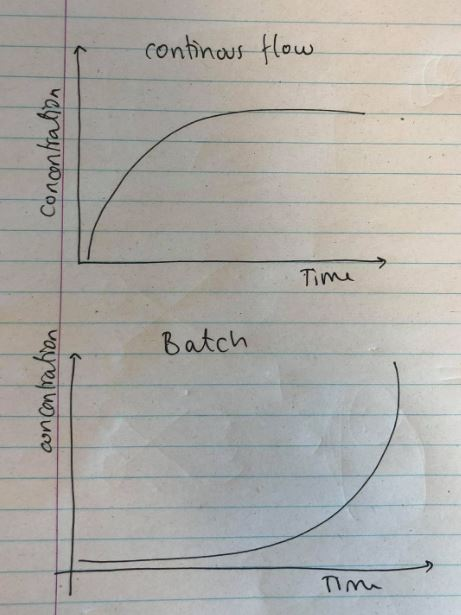
\includegraphics[width=0.4\textwidth]{Billeder/intro/continous_vs_batchflow.jpg}
	\caption{ sketch continuous flow vs. batch flow }
	\label{fig:continous_vs_batchflow}
\end{figure}

The problematic ions which constitute most of the make up water is \ce{Ca^{2+}}, \ce{Cl-}, \ce{SO_4^{2-}} and \ce{SiO2}.
Where \ce{SO_4^{2-}} (sulphate) is a good indicator for general conductivity in the thank and thus general rejection, see \cref{fig:sulphate_chlroide_concentration_batch} for concentration profile. 
Previous work (by Sebastian) have indicated problems with low rejection and also negative rejection for both \ce{Cl-} and \ce{SiO2}.

\textbf{Chloride}
\ce{Cl-} does not follow the same concentration profile as \ce{SO4} see \cref{fig:sulphate_chlroide_concentration_batch}, therefore other filtration protocols have been proposed in order to increase rejection. 
A method could be to lead only a certain partition of the permeate directly into the CT reservoir.
This first partition should be the region in which rejection of \ce{Cl-} was high , staying within the first partition of the concentration profile illustrated on \cref{fig:sulphate_chlroide_concentration_batch}. 
The second partition of permeate would be lead into other container which would be filtered again through the same NF membrane, but as the majority of \ce{SO_4^{2-}} ions have been removed, the \ce{Cl-} ions should continue to show high rejection. 




\begin{figure}[H] % (alternativt [htbp])
	\centering
	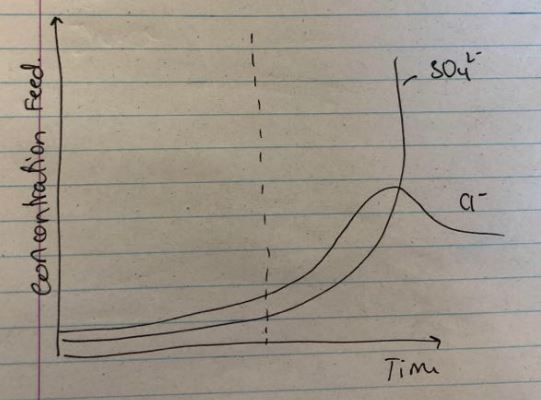
\includegraphics[width=0.5\textwidth]{Billeder/intro/sulphate_chloride_rejection.JPG}
	\caption{ sketch sulphate chloride concentratio in batch process}
	\label{fig:sulphate_chlroide_concentration_batch}
\end{figure}

\textbf{Silica}
With general NF treatment there is about 5-12\% rejection of \ce{SiO2}. Where uncharged \ce{SiO2} can pass the NF membrane, but charged \ce{SiO2} will be rejected similar to other negatively charged ions.
A way to increase the rejection of \ce{SiO2} can thereby be by increasing the pH level and thus control the charge of the \ce{SiO2}. 
The permeate is lead to a separate tank (apart from the very last feed), where the pH is raised from about pH 8 to pH 10.6 (a suggestion), and the is filtered again where the first half of permeate is introduced to the reservoir and the second half is discarded as blowdown water. 



The goal is to make a model based on experimental test, the model should be as simple as possible and should be able to make a suitable filtration method based on content of the makeup water / reservoir water. 
One way to developed the model could be the proposed fractional filtration proposed above in order to combat silica and chloride content respectively, where the exact partition of permeate should be investigated more in depth. 
The carbonate system should also be considered, and general interaction between the various ions. 
The model does not necessarily need to account for both high chloride and silica content, but the one which approach the guidelines, or which ever species is present in the makeup water. 

% \textbf{Experimental:} 

% Analysis methods: 
% \begin{itemize}
%     \item IC
%     \item Test kits for silica
% \end{itemize}

% Sensors: 
% \begin{itemize}
%     \item Conductivity
%     \item pH
%     \item Pressure
%     \item Thermometer
%     \item Chloride (not present, could be possibility)
%     \item Conductivity on membrane (not present, could be possible kristian) 
% \end{itemize}